\documentclass{article}
\usepackage{graphicx}
\usepackage{subcaption}
\usepackage{cleveref}
\usepackage{geometry}
\geometry{legalpaper, margin=1in}

\begin{document}
\noindent\textbf{1.} Compose a program to multiply two NxN matrices in C.\\
\indent See "matrixTemplate.c" and "matrixTemplate.h".\\

\noindent\textbf{2.} Create a script to generate six programs that will multiple the same matrices with identical data in six different (i,j,k) orders.\\
\indent See "program\_generator.py". I wrote a Python script to generate the six function of different (i,j,k) orders.\\

\noindent\textbf{3.} Verify that the outputs of six different matrix programs are identical.\\
\indent There is an int type varibale \texttt{check} in the "main.c". The program will compare the result of the six functions if \texttt{check} is set to 1.\\

\noindent\textbf{4.} Compose a script to harvest the running times of N=500 for the six different programs. Find the best performing order. Then run the best performing order for N=100, 200, 300, .., 1000.\\
\indent I use a loop to let the program run for all the N values.\\

\noindent\textbf{5.} Plot your results with explanations. There are two investigations: a) performance behavior for six orders, and b) performance behavior for different N.\\
    \begin{figure}[h!]
        \centering
        \begin{subfigure}[b]{0.3\linewidth}
          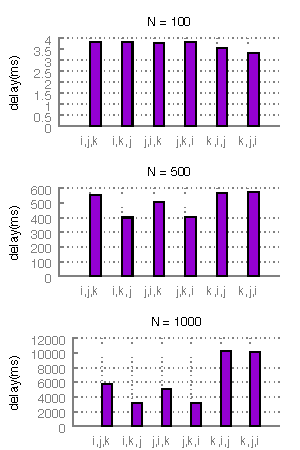
\includegraphics[width=\linewidth]{matrix_ijk.pdf}
          \caption{different i-j-k order}
          \label{fig:ijk}
        \end{subfigure}
        \begin{subfigure}[b]{0.3\linewidth}
          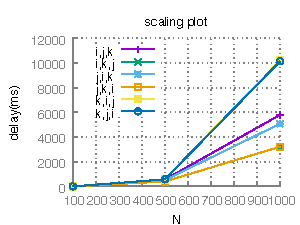
\includegraphics[width=\linewidth]{matrix_scaling.pdf}
          \caption{scaling}
          \label{fig:scaling}
        \end{subfigure}
        \caption{\label{fig:part1}}
    \end{figure}

\indent Figure. \ref{fig:part1} \subref{fig:ijk} shows the results for the six orders and Figure. \ref{fig:part1} \subref{fig:scaling} shows the result for the different N values. \\
\indent We can see that the order (i,k,j) and (j,k,i) have the best performance while the order (k,i,j) and (k,j,i) are worst. The difference is due to the special locality. When the matrix multiplication is calculated by the order (i,k,j) or (j,k,i), the program calculates the elements in the results one by one, without running back and forth, so the memory block holding the row or the column would not be loaded into CPU cache repeatedly. As for the order (k,i,j) and (k,j,i), they calculate all the elements of the result matrix at the same time, i.e., they loop over the memory blocks of the result matrix again and again until the calculation for all the elements has been calculated. And thus the memory block holding the row or column are loaded in to cache repeatedly. To sum up, each element in the result matrix requires \textbf{N multiplication operations}, and the order (i,k,j) and (j,k,i) will run the \textbf{N multiplication in a row}, while the the order (k,i,j) and (k,j,i) run \textbf{one multiplication each time for each element}, incurring overhead in reloading memory blocks holding the row and columns of the two multiplying matrices.\\
\indent As for the scaling, the order (i,k,j) is chose to run the program. As the N grows, the running times grows by the squere of N.
\end{document}
\Cref{fig:part1}
\Cref{fig:ijk}
\Cref{fig:scaling}